%Equation \ref{eq:dirac_comb_coeff} provides the formula for the phase and amplitude of each spectral component of a Dirac comb signal. What does this result tell you about how power is distributed over frequency?

%\item Using Section \ref{dirac_section}, implement a program that calculates a partial sum approximation of a Dirac delta train with period $T=0.5$ seconds. Use $N=50$ as the number of complex exponential signals to include in the partial sum. Evaluate the signal from t=0 to t=4 seconds at 10 kHz sample rate. Here's some partial code, which almost does the job. 
%\begin{lstlisting}[language=Python,numbers=none]
%# determine sample rate (Hz) sample_rate=10000.0 # create time array 0
%to 4 seconds t=n.arange(4.0*sample_rate)/sample_rate # initialize
%empty vector to hold Fourier series
%sig=n.zeros(len(t),dtype=n.complex) N=50 for k in range(-N,N): sig+=
%...
%    
%plt.plot(sig.real)
%plt.show()
%\end{lstlisting}
%\item[b)] Delay the signal by 0.1 seconds by applying a phasor term to the Fourier series coefficients, with the help of Section \ref{delay_section}. Plot the undelayed and delayed signals in the same plot and verify that the signal is delayed by the right amount.
%\end{itemize}

%\if
\newpage
\section{Variable star lightcurve fitting}
\newthought{Example: The study of astronomical light curves of variable stars is an example of a practical application of the Fourier series}.

Variable stars called Cepheids, have intensities $I(t)$ that varies
periodically as a function of time. An example of a light curve is
shown in Figure \ref{fig:cepheid_lightcurve}. Such variable stars
pulsate in luminosity in a regularly repeating manner. The repeating
luminosity waveform is often very non-sinusoidal, necessitating a
Fourier series analysis.

\begin{marginfigure}
\begin{center}
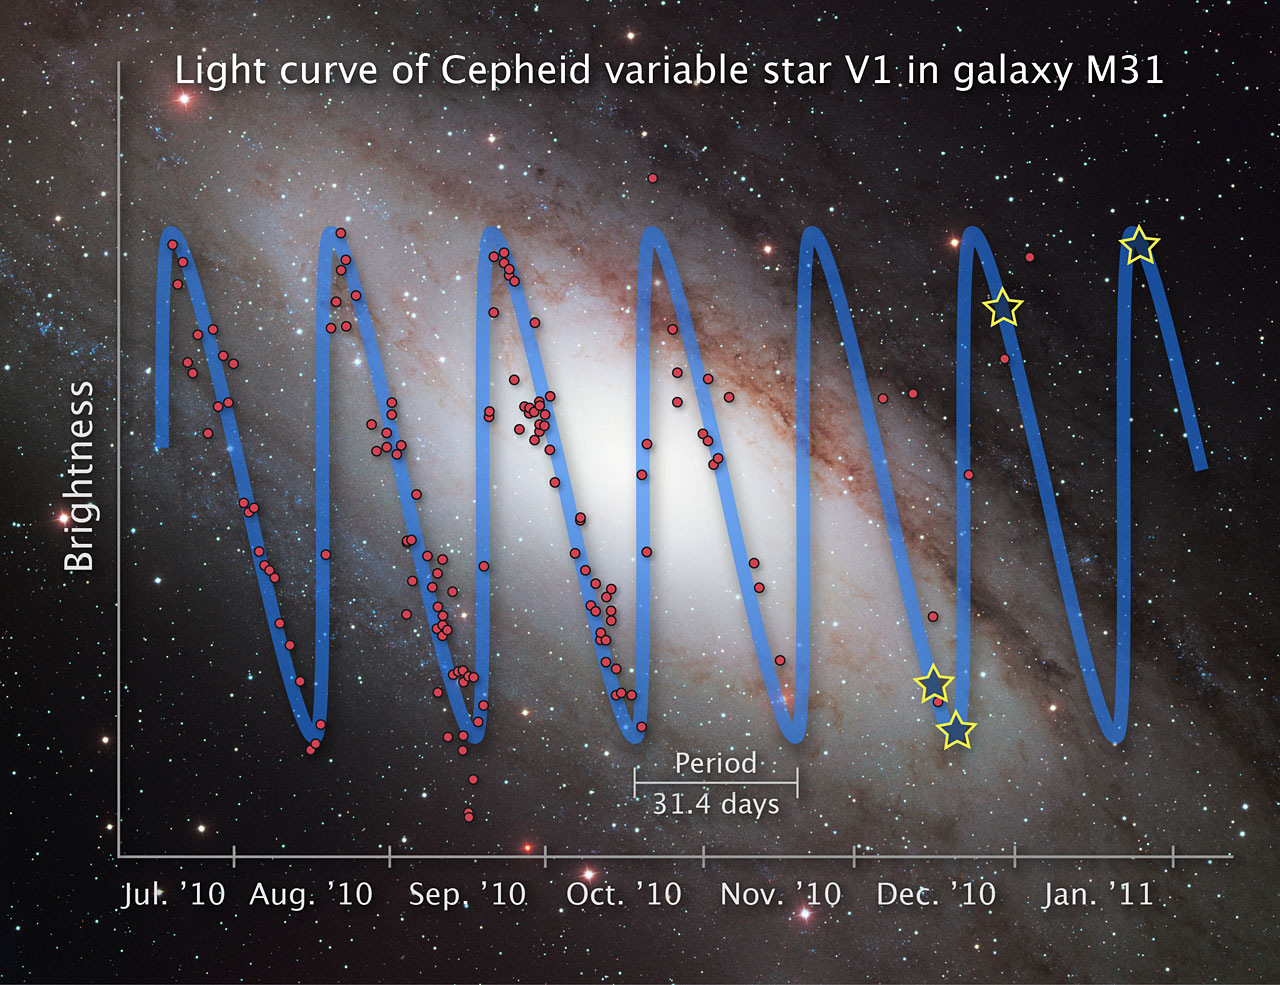
\includegraphics[width=\textwidth]{Applications/figures/ceph.jpg}
\end{center}
\caption{Measurements of the intensity of a variable star (red) and a Fourier series model of the intensity of the star as a function of time (blue). Illustration Credit: NASA, ESA and Z. Levay (STScI). Science Credit: NASA, ESA, the Hubble Heritage Team (STScI/AURA) and the American Association of Variable Star Observers.}
\label{fig:cepheid_lightcurve}
\end{marginfigure}

Measurements of the intensity of a Cepheid variable star are made at
periods of time when telescope time is available and astronomical
seeing allows observations to be made. The time spacing between
measurements is therefore by no means regular.

When analyzing the periodic waveform of this star, a search is made to
determine the period $T$ of the intensity waveform, and the Fourier
series coefficients $c_k$. This is done by using an exhaustive search
for plausible values of $T$. The model function is a Fourier series
synthesis equation:
\begin{equation}
I_N(t) = \sum_{k=-N}^N c_k e^{i\frac{2\pi}{T}kt} \,\,.
\end{equation}
The relationship between absolute brightness and the pulsation
frequency (fundamental frequency) is thought to be relatively
stable. This makes these types of variable stars useful for measuring
the astronomical distances.


The Fourier series can be used to express periodic functions. One real
life use case is estimating the functional form for a periodic star,
which varies in brightness periodically. In this exercise, we will
determine the Fourier series coefficients for brightness observations
of a real Cepheid star. We will then plot the Fourier series for the
periodic light curve of this star.

To estimate the periodic waveform for a Cepheid variable star
brightness measurements $m(t)$, we will use something called the
maximum likelihood method, which estimates the Fourier series
coefficients.  This involves expressing the Fourier series as a matrix
vector operation:
\begin{align}
m &= A x\\
\begin{bmatrix}
m(t_0)\\
m(t_1)\\
m(t_2)\\
\vdots \\
m(t_{M})
\end{bmatrix} &=
\begin{bmatrix}
e^{i\frac{2\pi}{T} k_0 t_0} & e^{i\frac{2\pi}{T} k_1 t_0} & \hdots & e^{i\frac{2\pi}{T} k_N t_0} \\
e^{i\frac{2\pi}{T} k_0 t_1} & e^{i\frac{2\pi}{T} k_1 t_1} & \hdots & e^{i\frac{2\pi}{T} k_N t_1} \\
\vdots & \vdots & \ddots & \vdots \\
e^{i\frac{2\pi}{T} k_0 t_M} & e^{i\frac{2\pi}{T} k_1 t_M} & \hdots & e^{i\frac{2\pi}{T} k_N t_M} 
\end{bmatrix} 
\begin{bmatrix}
c_0 \\
c_1 \\
c_2 \\
\vdots \\
c_N
\end{bmatrix}  \,\,.
\end{align}
Here $c_k$ is a Fourier series coefficient and $T$ is the fundamental
period. Because there are discrete measurements, the measurement
function is only known at discrete points $m(t_{\ell})$. In order to
estimate the Fourier series coefficients, we use the linear
least-squares estimator:
\begin{equation}
\hat{x} = (A^H A)^{-1}A^H m \,\,.
\end{equation}
The vector $\hat{x}$ will now contain the most probable Fourier series
coefficients that explain the measurements $m(t_{\ell})$ of the
periodic function.

Because this course does not deal with statistics, we have implemented
the code that figures out the Fourier series coefficients that fit the
measurements. Your task is to edit the code below, and to evaluate the
Fourier series model, given the coefficients $c_k$, which are in the
array variable named \verb|c_k|. Code is shown in Listing
\ref{lst:variable_star}, which already does most of the work. Complete
the last for-loop, and you should get the following plot:
\begin{center}
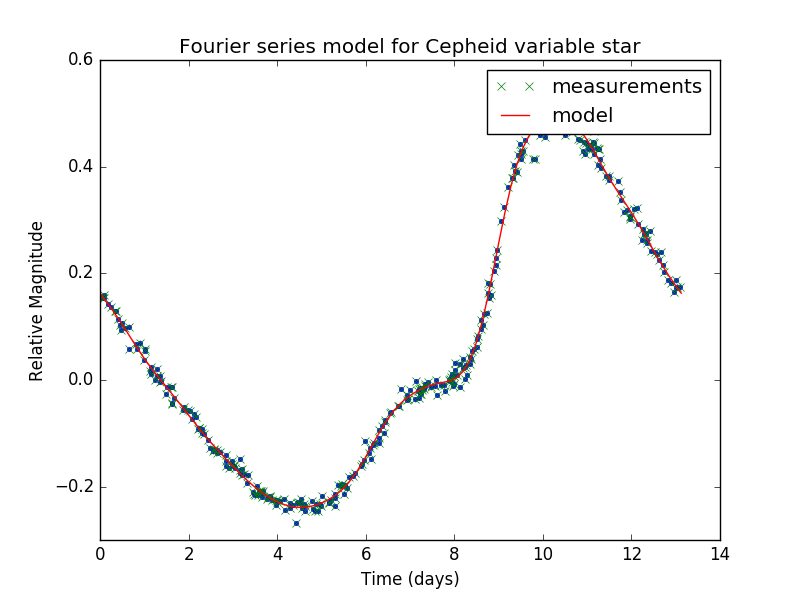
\includegraphics[width=0.92\textwidth]{Applications/figures/ceph.png}
\end{center}

\lstinputlisting[language=Python,caption={\texttt{012\_variable\_star/variable\_star.py}},label=lst:variable_star]{code/012_variable_star/variable_star.py}


